\section{Stochastic Simulation}
\label{ch:stochsim}
Another, more recently proposed way of simulating chemical systems are stochastic simulation algorithms (SSA) \cite{gillespie_general_1976}. Unlike in the deterministic case, the solution obtained is not unique, but it only represents one possible way the system can develop in time. In theory, i.e.\ on a computer with infinite precision equipped with a perfect source of random numbers, the probability that a SSA will give exactly the same result in two or more independent runs is zero. In practice, however, a computer is a highly deterministic machine with finite precision. Therefore, the number of possible solutions of a SSA is finite. Since most computers don't have true random generators built in, pseudo-random number generators (PRNG) have to be used. PRNGs can create a sequence of numbers $Z_i$ that is random in the sense that it is compliant with a given probability distribution (usually $Z \sim \mathcal{U}(0,1)$) according to a variety of statistical tests (i.e.\ the TestU01 Big Crush testing battery(cite!)). However, a PRNG is completely defined by its state structure so that for a given state, the sequence of numbers generated thereafter is deterministic. The initial state is usually derived from a seed value. If a SSA is run with a fixed seed value, its output will always be the same. From now on, for the sake of simplicity, the terms "random number generator" and "random number" will be used as synonyms for "pseudo-random number generator" and "pseudo-random number", respectively. 

Compared to the deterministic approach towards simulating chemical reaction systems, the stochastic approach is computationally more demanding. The main reason for this is the high expense at which random numbers are generated on a computer. Despite this disadvantage, the demand for good SSAs in research and industry has been on the rise over the past decade. For a large number of particles of every species in the system, it can be shown that the two approaches are identical, for low particle counts, however, this is not the case. Especially in biochemistry and genetics, some systems are described insufficiently by traditional deterministic models. Often particles which dominate the dynamic behavior of the system are only present in small numbers. In such situations, SSAs are an important tool to enable a more detailed understanding of the system. Noise introduced by the randomness of microscopic processes such as Brownian motion cannot be neglected but is an integral factor that determines system behaviour in practice. 

%\subsection{Definitions}
\subsection{Definitions} % Remove?
\label{ch:def_stoch}
Let there be a chemical reaction system with species $X_i$, $i=1, \ldots,N$ and reactions $R_j$, $j=1, \ldots,M$. Now, the state of the system $\vec{x}(t)$ at time $t$ is determined by the number of particles $x_i$ of the species $X_i$, i.e.\ $\vec{x}(t) = \begin{bmatrix} x_1(t) & x_2(t) & \ldots & x_N(t)\end{bmatrix}^T$. The initial state of the system at time $t_0$ is $\vec{x}_0 = \vec{x}(t_0)$. The state change vector $\vec{\nu_j}$ of reaction $R_j$ is defined such that when the reaction takes place, the state of the system changes from $\vec{x}$ to $\vec{x} + \vec{\nu}_j$. The $i$-th component of the state change vector gives the number of particles that are consumed ($\nu_{ij} < 0$) or created ($\nu_{ij} > 0$) when reaction $R_j$ occurs. Again, we will only consider spatially homogeneous (i.e.\ well-stirred) systems in the beginning. 

The fundamental assumption of the deterministic description is that the probability of reaction $R_j$ taking place during the time interval $\lbrack t, t + dt)$ is (cite!)
\begin{align}
\label{eq:assumption}
\alpha_j(\vec{x}(t)) \, dt + \mathcal{O}(dt^2)
\end{align}

The propensity function $\alpha_j$ of reaction $R_j$ is dependent on the state of the system $\vec{x}(t)$. In its most general form, it is given as
\begin{align}
\label{eq:propensity}
\alpha_j(\vec{x}(t)) = \Omega k_j \prod_{i=1}^N \binom{x_i}{r_{ij}} \Omega^{-r_{ij}}
\end{align}
where $k_j$ is the reaction rate of reaction $R_j$, $x_i$ the number of molecules of species $X_i$ at time $t$. Reaction $R_j$ consumes $r_{ij}$ molecules of species $X_i$. The binomial coefficient $\binom{n}{k} = \frac{n!}{k!\,(n-k)!}$ gives the number of distinct subsets of size $k$ from a set of size $n$. In the context of chemical reactions this is the number of different scenarios that can occur when a reaction requires the collision of $k$ out of $n$ available particles. $\Omega$ is the number of molecules per volume unit associated to unit concentration in the deterministic model. Chapter \ref{ch:scaling} gives a detailed explanation of why this scaling factor is needed. 

Considering the local reactions from the Gray-Scott model, one gets the following propensity functions: \par
Generation of U \eqref{eq:r1}:
\begin{align}
\alpha_1 = F \Omega
\end{align}
Degradation of U \eqref{eq:r2}
\begin{align}
\alpha_2 = F u
\end{align}
Degradation of V \eqref{eq:r3}
\begin{align}
\alpha_3 = (F + \kappa) v
\end{align}
Autocatalytic Conversion \eqref{eq:r4}
\begin{align}
\alpha_4 = \rho \frac{u v (v-1)}{2 \Omega^2}
\end{align}
\paragraph{Remark:} (Work in progress!) Be careful about the 2! Limit of propensity formula, $\Omega$, equivalence of both models. In order to simulate the same system, the parameter $\rho = 1.0$ in the deterministic model corresponds to $\rho = 2.0$ in the stochastic case.

%\subsection{Chemical Master Equation}
\subsection{Chemical Master Equation}
The following derivations are based on ideas presented in \cite{lipkova_stochastic_2011}. Reconsidering equation \eqref{eq:assumption}, the probability that a reaction $R_j$ with propensity function $\alpha_j$ takes place in a time interval $\lbrack t, t+dt)$ is approximately $\alpha_j dt$. Let the time step $dt$ be short enough such that the probability of $R_j$ occurring more than once during the interval is negligible. Then the conditional probability of the system being in state $\vec{x}$ at time $t+dt$ given that it was in state $\vec{x_0}$ at time $t_0$ is
\begin{align}
\begin{split}
\label{eq:diffquot}
\mathcal{P}(\vec{x},t+dt|\vec{x}_0,t_0) &= \mathcal{P}(\vec{x},t|\vec{x}_0,t_0) \lbrack 1 - \sum_{j=1}^M \alpha_j(\vec{x}) dt \rbrack \\
&+ \sum_{j=1}^M \mathcal{P}(\vec{x} - \vec{\nu}_j,t|\vec{x}_0,t_0) \,\alpha_j(\vec{x} - \vec{\nu}_j) dt
\end{split}
\end{align}
The first term of the equation represents the case where the system is in state $\vec{x}$ at time $t$ and no reactions take place in the interval $\lbrack t,t+dt)$. The second term takes account for the cases where exactly one of the $M$ reactions occurs. The system must have been in the state $\vec{x} - \vec{\nu}_j$ at time $t$ to reach the state $\vec{x}$ after the firing of $R_j$. 

By rearranging equation \eqref{eq:diffquot} a difference quotient can be obtained. Passing the limit $dt \rightarrow 0$ yields the Chemical Master Equation (CME):
\begin{align}
\begin{split}
\frac{\partial}{\partial t} \mathcal{P}(\vec{x},t|\vec{x}_0,t_0) &= \sum_{j=1}^M \mathcal{P}(\vec{x}-\vec{\nu}_j,t|\vec{x}_0,t_0) \,\alpha_j(\vec{x} - \vec{\nu}_j) \\
&- \sum_{j=1}^M \mathcal{P}(\vec{x},t|\vec{x}_0,t_0) \,\alpha_j(\vec{x})
\end{split}
\end{align}
The CME of the homogeneous Gray-Scott model in the state $\vec{x} = \begin{bmatrix} U & V\end{bmatrix}^T$ is
\begin{align}
\begin{split}
\frac{\partial \mathcal{P}(U,V)}{\partial t} &= F \Omega \cdot \mathcal{P}(U-1,V) \\
&+ (U+1)F \cdot \mathcal{P}(U+1,V) \\
&+ (V+1) (F+\kappa) \cdot \mathcal{P}(U,V+1) \\
&+ \rho \frac{(U+1) (V-1) (V-2)}{2\Omega^2} \cdot \mathcal{P}(U+1,V-1) \\
&- \left(F\Omega + UF + V(F+\kappa) + \rho \frac{UV(V-1)}{2\Omega^2}\right) \cdot \mathcal{P}(U,V)
\end{split}
\end{align}
$\mathcal{P}(U,V)$ is used as an abbreviation for $\mathcal{P}(U,V,t|U_0,V_0,t_0)$. 

The solution of the CME of a system with initial conditions $\vec{x}_0 = \vec{x}(t_0)$ gives the conditional probability $\mathcal{P}(\vec{x},t|\vec{x}_0,t_0)$ that the state of the system is $\vec{x}$ at time $t$. Since the number of molecules in the system is in general not limited (i.e.\ in the Gray-Scott model nothing stops reaction \eqref{eq:r1} from creating  U particles), the dimension of the system of ODEs is infinite. In practice, an exact solution can only be obtained for some simple systems. Therefore, in the next chapter a computational algorithm of great practical importance will be presented. 
%
%

%\subsection{Gillespie Algorithm}
\subsection{Gillespie Algorithm}
The Chemical Master Equation presented in the previous chapter gives an exact description of the time evolution of a chemical reaction system. In practice, however, it is impractical (or even impossible) to obtain the solve explicitly. Since it is based on the same basic assumptions, the Gillespie Algorithm is a simulation method that is equivalent to the CME. However, the approach does not try to solve the equation explicitly, but simulates the underlying Markov process the CME describes analytically. The main idea of the algorithm can be summarized by two questions that have to be answered in every simulation step: "What is the next reaction that takes fires?" (i.e.\ what is the next state of the system) and "When will this happen?" (i.e.\ at what time will the state transition take place). In the following the Gillespie SSA will be derived based on basic probability theory concepts. 

Let there be a chemical reaction system with species $X_i$, $i=1, \ldots,N$ and reactions $R_j$, $j=1, \ldots,M$. The state of the system $\vec{x}(t)$ at time $t$ is determined by the number of particles $x_i$ of the species $X_i$. The initial state of the system at time $t_0$ is $\vec{x}_0 = \vec{x}(t_0)$. The state change vector $\vec{\nu_j}$ of reaction $R_j$ is defined such that when the reaction takes place, the state of the system changes from $\vec{x}$ to $\vec{x} + \vec{\nu}_j$. The $i$-th component of the state change vector gives the number of particles that are consumed ($\nu_{ij} < 0$) or created ($\nu_{ij} > 0$) when reaction $R_j$ occurs. In the following derivation, for the sake of readability, the dependency of the propensity functions $\alpha_j$ on the state of the system $\vec{x}(t)$ will be omitted.

For the moment, just a single reaction $R_j$ of the system equipped with the propensity function $\alpha_j$ is considered. Let $f_{0,j}(\tau+d\tau)$ be the probability that the reaction does not fire in the time interval $\lbrack t,t+\tau+d\tau)$, where $d\tau$ is an infinitesimal time step and $\tau > 0$. This is equivalent to the formulation that $R_j$ does not occur in the interval $\lbrack t,t+\tau)$ and in the subsequent instant $(t+\tau+d\tau)$:
\begin{align}
f_{0,j}(\tau + d\tau) = f_{0,j}(\tau) \cdot (1-\alpha_j d\tau). 
\end{align}
Rearranging and passing the limit of $d\tau \to 0$ leads to
\begin{align}
\lim_{d\tau \to 0} \frac{f_{0,j}(\tau + d\tau) - f_{0,j}(\tau)}{d\tau} = \frac{df_{0,j}(\tau)}{d\tau} = -\alpha_j f_{0,j}(\tau)
\end{align}
Solving the differential equation with the initial condition $f_{0,j}(0) = 1$ yields
\begin{align}
\label{eq:probnot}
f_{0,j}(\tau) = \exp(-\alpha_j \tau)
\end{align}

Considering the complete system, in the case that none of the $M$ reactions of the system fires in the interval $\lbrack t,t + \tau)$, one has
\begin{align}
\begin{split}
f_0(\tau) &= \mathcal{P}(\tau_1 > \tau \wedge \tau_2 > \tau \wedge \ldots \wedge \tau_M > \tau) \\ 
&= \mathcal{P}(\min (\tau_j) > \tau) = \prod_{k=1}^M \alpha_k\exp(-\alpha_k \tau) \\ 
&= \exp(-\alpha_0 \tau)
\end{split}
\end{align}
where $\alpha_0 = \sum_{k=1}^M \alpha_k$. 

The probability density $f_1(\tau)$ that any reaction fires at time $t+\tau$ is given by the probability that none fired in the interval $\lbrack t,t+\tau)$ and the probability that exactly one fires in the instant $(t+\tau)$:
\begin{align}
f_1(\tau) = \exp(-\alpha_0 \tau) \cdot \alpha_0
\end{align}
The waiting time $\tau$ until any reaction $R_j$, $j=1,\ldots,M$ fires is therefore exponentially distributed, i.e.\ $\tau \sim \operatorname{Exp}(\alpha_0)$. The corresponding cumulative distribution function (CDF) is given by
\begin{align}
F(\tau) = \int_0^\tau f_1(t) dt = 1 - \exp(-\alpha_0 \tau)
\end{align}
Since most random number generators can only generate random numbers $r_1 \sim \operatorname{Unif}(0,1)$, inverse probability integral transform (cite the paper!!!) can be used to generate $\tau \sim \operatorname{Exp}(\alpha_0)$:
\begin{align}
\tau = F^{-1}(r_1) = \frac{1}{\alpha_0} \ln\left(\frac{1}{1-r_1}\right)
\end{align}
In this case, the (excluded) values $r_1=0$ and $r_1 = 1$ are mapped to $\tau = 0$ and $\tau = \infty$, respectively. A computationally favorable but otherwise equivalent mapping is
\begin{align}
\tau = \frac{1}{\alpha_0} \ln \left( \frac{1}{r_1} \right)
\end{align}
where $r_1=0$ and $r_1=1$ are mapped to $\tau = \infty$ and $\tau = 0$. Considering only the real part of the complex logarithm, it can be obtained by moving the original function to the left by $1$ (i.e.\ $r'=r+1$) and then mirroring it on the ordinate axis. Figure \ref{fig:inversetransform} illustrates this process. 
\begin{figure}
\centering
\includegraphics[width=\textwidth]{images/inversetransform.eps}
\caption{Inverse probability integral transform: original mapping drawn in blue, modified function in red. Solid lines are used in the domain of interest, dashed ones illustrate the symmetry of the function (imaginary parts omited). Asymptotes are indicated by dots.}
\label{fig:inversetransform}
\end{figure}

Now that a way to find the time $\tau$ when the next reaction takes place has been derived, the next step is to determine which reaction actually fired. This, however, is straightforward: 

Let $r_2$ be a random number uniformly distributed in the interval $(0,1)$, i.e.\ $r_2 \sim \operatorname{Unif}(0,1)$. Then $R_j$ is the reaction which fired in the interval $\lbrack t,t+\tau)$ if the index $j$ fulfills
\begin{align}
\label{eq:nextr}
\frac{1}{\alpha_0} \sum_{k=1}^{j-1} \alpha_k \leq r_2 < \frac{1}{\alpha_0} \sum_{k=1}^{j} \alpha_k
\end{align}

Combining the results from above, the Gillespie Algorithm can be outlined as follows: \\
\begin{framed}
\begin{algorithm}[H]
\DontPrintSemicolon
\KwIn{Initial state $\vec{x}_0$, propensity functions $\alpha_j$, time $t_{end}$}
\KwOut{State $\vec{x}(t)$ for $t \in \lbrack t,t_{end}\rbrack$}
 \textbf{Initialization:} Set time $t = 0$ and state $\vec{x} = \vec{x}_0$.\;
 \While{$t < t_{end}$}{
  Generate random numbers $r_1,r_2 \sim \mathcal{U}(0,1)$.\;
  \For{$j = 1$ \KwTo $M$}
  {
  Compute the propensity function $\alpha_j(\vec{x})$.\;
  }
  Compute the sum of all propensities $\alpha_0 = \sum_{j=1}^M \alpha_j$.\;
  Compute the time step $\tau = \frac{1}{\alpha_0} \ln \left( \frac{1}{r_1} \right)$.\;
  Find $j \in \lbrack1,M\rbrack$ such that $\sum_{k=1}^{j-1} \alpha_k \leq r_2 \alpha_0 < \sum_{k=1}^j \alpha_k$ holds.\;
  Set $\vec{x} = \vec{x} + \vec{\nu}_j$.\;
  Set $t = t + \tau$.\;
 }
 \caption{Gillespie Algorithm}
\end{algorithm}
\end{framed}

Figure \ref{fig:gs_time_evolution} shows three independent Gillespie SSA samplings of the temporal evolution of the well-stirred Gray-Scott model. The number of molecules is rescaled to obtain concentrations, the factor $\Omega = 1000$ was used (see chapter \ref{ch:scaling}). Reaction constants are $F=0.04$, $\kappa = 0.06$ and $\rho_s = 2.0$. The initial condition is given as $u_0=500$ and $v_0 = 250$ which is equivalent to initial concentrations of 0.5 and 0.25, respectively. The dashed line indicates the deterministic solution obtained numerically using a fifth-order Runge-Kutta scheme. In Figure \ref{fig:gs_hist_10} a histogram of the number of U molecules at time $t=10$ is shown. The results from 100000 samples are partitioned in 30 bins. 

\begin{figure}
\centering
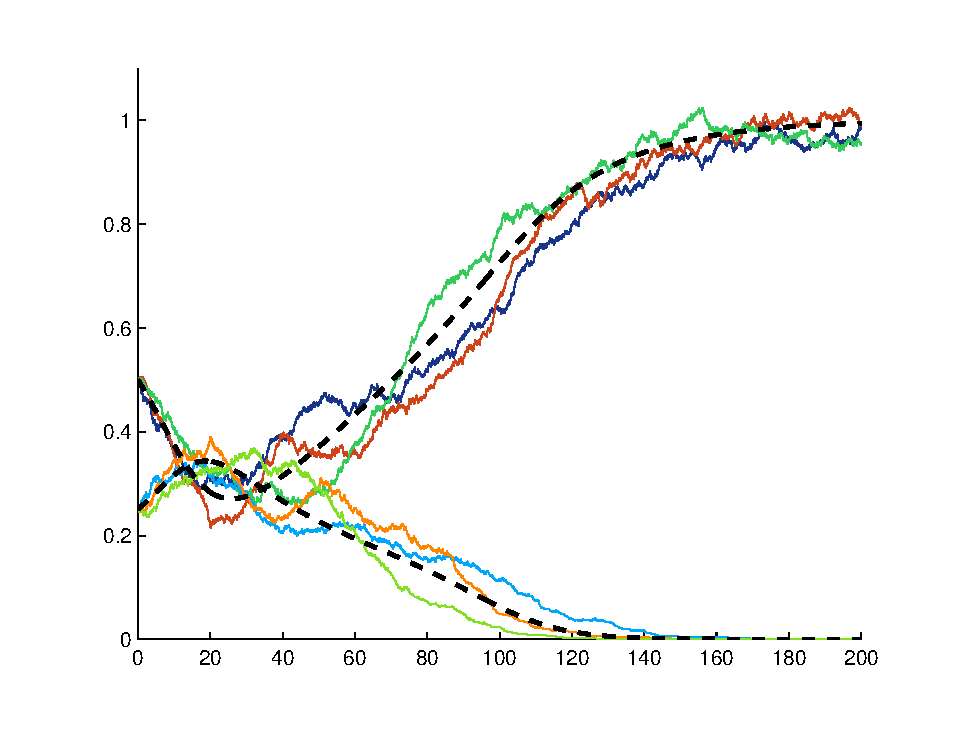
\includegraphics[width=\textwidth]{images/gs_time_evolution.eps}
\caption{Stochastic simulation of the well-stirred Gray-Scott model with $F=0.04$, $\kappa=0.06$, $\rho_s = 2.0$, $u_0=500$ and $v_0=250$. The concentrations ($\Omega=1000$) of both species over times ($t\in[0,200]$)is plotted. Color codeing: dark colors represent species U, bright colors represent species V.}
\label{fig:gs_time_evolution}
\end{figure}

\begin{figure}
\centering
\includegraphics[width=\textwidth]{images/gs_hist_10.eps}
\caption{Histogram obtained by 100000 Gillespie SSA samples evaluated at $t=10$. Parameters and initial conditions similar to figure \ref{fig:gs_time_evolution}}
\label{fig:gs_hist_10}
\end{figure}

\ifdebug
Algorithm (derivation from Oxford Paper)
Leaping condition, tau formula\cite{cao_adaptive_2007}
\begin{itemize}
\item Exact method
\item you can compare time evolution of concentration/number of a specie from deterministic and stochastic simulation 
\item often mean of stochastic realization correspond to deterministic solution, but it is not a rule, but it is nice to show that in the limit of large number of molecules stochastic solution converge to deterministic one
\item A lot of improvements were proposed but it is still computational expensive/prohibitive. 
\end{itemize}
\fi

%\subsection{Tau-leaping Algorithm}
\subsection{Tau-leaping Algorithm}
\ifdebug
Be careful about probability and probability density!!! \\
\fi
The Gillespie Algorithm presented in the previous chapter enables exact numerical simulations of well-stirred chemical reaction systems. It takes account for the inherent randomness in such systems and obeys the same microphysical principles that underlay the Chemical Master Equation. In addition, the algorithm is relatively easy to implement. In practice, however, it turns that even for moderately-sized systems the computational costs of applying the Gillespie algorithm are prohibitive. This is especially true for real-world applications where not just one single trajectory is needed, but a great number of samples must be obtained to estimate probability densities. For every single reaction the system needs to be updated and (some) propensity values have to be recalculated. Consequently, the temporal evolution is obtained up to a level of detail that is neither useful nor necessary for typical applications. It is obvious that there is a need for accelerated (parallelizable) stochastic simulation algorithms. 

In the following, the tau-leaping algorithm originally proposed in \cite{gillespie_approximate_2001} is presented. "By making a minor sacrifices in simulation accuracy, major gains in performance can bet obtained." Considering the overall principle of the algorithm, a clear similarity to the explicit Euler method applied to deterministic models can be observed. 

Equation \eqref{eq:probnot} in the previous chapter gives the probability that a reaction $R_j$ does not fire in an interval $\lbrack t,t+\tau)$. The probability density that it fires in the instant $t+\tau$ is
\begin{align}
f_{1,j}(\tau) = f_{0,j}(\tau) \cdot \alpha_j = \alpha_j \exp(-\alpha_j \tau)
\end{align}
The time one has to wait until reaction $R_j$ fires is therefore exponentially distributed, i.e.\ $\tau \sim \operatorname{Exp}(\alpha_j)$. Without loss of generality, due to the memorylessness of the exponential distribution, i.e.\ $\mathcal{P}(\tau > t + s|\tau > t) = \mathcal{P}(\tau > s)$ the interval $\lbrack0,\tau)$ can be considered. Let $k$ be the number of times the reaction takes place in this interval. Then the probability that $R_j$ fires exactly zeros times is
\begin{align}
\begin{split}
\mathcal{P}(k=0) = \int_\tau^\infty f_{1,j}(t) dt =
\int_\tau^\infty \alpha_j \exp(-\alpha_j t) dt = \exp(-\alpha_j \tau)
\end{split}
\end{align}
The probability that $R_j$ fires exactly once in the interval is
\begin{align}
\begin{split}
\mathcal{P}(k=1) &= \int_0^\tau f_{1,j}(x) \left( \int_{\tau-x}^\infty f_{1,j}(t) dt \right) dx \\
&= \int_0^\tau \alpha_j \exp(-\alpha_j x) \left( \int_{\tau-x}^\infty \alpha_j \exp(-\alpha_j t) dt \right) dx \\
&= \alpha_j \tau \exp(-\alpha_j \tau)
\end{split}
\end{align}
where $x \in \lbrack 0,\tau)$ is the time when $R_j$ actually fires. The inner integral gives the probability that the reaction does not fire thereafter. 

The probability that $R_j$ fires exactly twice in the interval is 
\begin{align}
\begin{split}
\mathcal{P}(k=2) &= \int_0^\tau f_{1,j}(x) \left( \int_x^\tau f_{j,1}(y) \left( \int_{\tau-x-y}^\infty f_{1,j}(t)dt \right) dy \right) dx \\
&= \frac{(\alpha_j \tau)^2}{2} \exp(-\alpha_j \tau)
\end{split}
\end{align}
It can be shown that for arbitrary $l \in \mathbb{N}_0$ the following formula for the probability of counting exactly $l$ firings in the interval is (cite Grimmett, pg. 247, 248)
\begin{align}
\mathcal{P}(k=l) = \frac{(\alpha_j \tau)^l}{l!} \exp(-\alpha_j \tau)
\end{align}
The number of times reaction $R_j$ takes place in the interval $\lbrack 0,\tau)$ is therefore Poisson distributed, i.e.\ $l \sim \operatorname{Pois}(\alpha_j \tau)$. This result is the main idea used in the tau-leaping algorithm. 

Up to now, the implicit assumption that $\alpha \ne \alpha(\vec{x}(t))$ was made. Reconsidering equation \eqref{eq:propensity}, this is not the case. After each firing of a reaction the state changes and so do (in general) the propensities. For the tau-leaping algorithm, however, the assumption is made that the propensities remain approximately constant during a time interval of length $\tau$. Mathematically this can be formulated as follows:
\begin{align}
\abs{\alpha_j(\vec{x}(t+\tau)) - \alpha_j(\vec{x}(t))} \leq \epsilon \alpha_0(\vec{x}(t))
\end{align}
where $0 < \epsilon \ll 1$ is a parameter defined by the user to control model accuracy.  

If this so-called Leap Condition (cite Gillespie) is satisfied, the number of firings for each of the $M$ reactions can be approximated by a Poisson random variable with mean $\alpha_j \tau$. The state of the system at time $t + \tau$ is
\begin{align}
\vec{x}(t+\tau) = \vec{x}(t) + \sum_{j=1}^M k_j \vec{\nu}_j
\end{align}
where $k_j \sim \operatorname{Pois}(\alpha_j \tau)$.

The task of finding a suitable $\tau$, however, is nontrivial. A time step that is too long makes the simulation inaccurate, one that is too short increases computing time. Over the years a variety of different procedures have been proposed (cite some). One of the most sophisticated $\tau$-selection formulas is described in (Cao et al. from R-leap). It is given as follows:
\begin{align}
\label{eq:tau}
\tau = \min\left\{ \frac{\max \left\{ \frac{\epsilon x_i(t)}{g_i}, 1\right\}}{\abs{\mu_i(\vec{x}}}, 
\frac{\max \left\{ \frac{\epsilon x_i(t)}{g_i}, 1 \right\}^2}{\abs{\sigma_i^2(\vec{x}}} \right\}
\end{align}
where $I_{rs}$ is the set of all reactant species in the system. For these species the parameter $g_i$ is defined as follows:
\begin{align}
g_i = h_i + \frac{h_i}{n_i} \sum_{j=1}^{n_i-1} \frac{j}{x_i(t) - j}
\end{align}
$h_i$ denotes the highest order of reaction in which species $X_i$ appears as a reactant, $n_i$ is the number of $X_i$ molecules that are consumed in any of the highest order reactions (Check with 19 of R-leaping paper). The terms $\mu_i$ and $\sigma_i^2$ are given by 
\ifdebug
(What do $\mu$ and $\sigma$ mean?)
\fi
\begin{gather}
\mu_i(\vec{x}) = \sum_{j=1}^M \nu_{ij} \alpha_j(\vec{x}) \\
\sigma_i^2(\vec{x}) = \sum_{j=1}^M \nu_{ij}^2 \alpha_j(\vec{x})
\end{gather}

\paragraph{Remark: Negative populations}
Due to the unboundedness of the Poisson distribution, it can happen that in a leaping step more molecules are consumed than there are available in the system. The resulting negative population of the species is unphysical since the system cannot be in such a state in reality. A lot of different measures to avoid this problem have been proposed (e.g.\ \cite{cao_avoiding_2005, anderson_incorporating_2008}). For this thesis, however, the simplest resolution strategy is chosen: A step which creates negative populations is rejected, the proposed tau is reduced, e.g.\ $\tau_{new} = \tau_{old} / 2$. 
\newpage

The tau-leaping algorithm can be outlined as follows: 

\begin{framed}
\begin{algorithm}[H]
\DontPrintSemicolon
\KwIn{Initial state $\vec{x}_0$, propensity functions $\alpha_j$, time $t_{end}$}
\KwOut{State $\vec{x}(t)$ for $t \in \lbrack t,t_{end}\rbrack$}
 \textbf{Initialization:} Set time $t = 0$ and state $\vec{x} = \vec{x}_0$.\;
 \While{$t < t_{end}$}{
  \For{$j = 1$ \KwTo $M$}
  {
  Compute the propensity function $\alpha_j(\vec{x})$.\;
  }
  Compute the time step $\tau$ according to \eqref{eq:tau}.\;
  \For{$j = 1$ \KwTo $M$}
  {
  Generate a random number $k_j \sim \operatorname{Pois}(\alpha_j \tau)$, i.e.\ the number of time reaction $R_j$ fires.\;
  }
  \If{any of the populations would be negative}{
   Set $\tau = \tau / 2$\;
   Continue at the beginning of the loop\;
   }
  Set $\vec{x} = \vec{x} + \sum_{j=1}^M k_j \vec{\nu}_j$.\;
  Set $t = t + \tau$.\;
 }
 \caption{Tau-leaping Algorithm}
\end{algorithm}
\end{framed}

By leaping over a different time slots instead of considering every individual reaction the computational effort of stochastic simulations can be reduced significantly. The losses in simulation accuracy must be considered, but usually remain within a tolerable range. In the next chapter parallel implementations for multi-core CPU and GPU of the tau-leaping algorithm derived above will be presented. 

\mbox{\color{red}{solve gray-scott and compare to SSA}}

\ifdebug
\begin{itemize}
\item Exact since they generate statistically exact sample paths. Typically, one generates many sample paths (Ausprägungen) to approximate the underlying probability distribution of the system of interest. 
\item But this doesn't work for most systems, since it is computationally too expensive. 
\item Although progress has been made, an exact procedure that simulates every reaction is too inefficient for most realistic problems. 
\item One large population blocks simulation, stiffness, timescales, doesn't influence dynamics of system

\item Approximate method: Major gains in simulation speed obtained by minor sacrifices in simulation accuracy. 
\item Outperforms SSA: Several reactions per step
\item Assumption: Propensity functions $\alpha_k(X(t))$ are relatively constant in a short time interval $(t,t+\tau)$. 
\item Similar to explicit Euler method. Natural connection between SSA in stochastic regime and explicit Euler method applied to the chemical Langevin equation. 
\item Question: How to select the tau?
\item If time-step is too small, then use explicit SSA (Gillespie)
\item Problem: Negative populations --> Solutions proposed in ...
\item How to avoid? R-leaping, SSA for critical reactions
\item Stiffness: Presence of multiple timescales in the system
\item you can plot histogram (pdf for a number of molecules of some specie at some fix time) for different values of parameter epsilon and compare them with histogram from Gillespie
\item this shows what is the role of epsilon
\item To do it, use some non-stiff system, otherwise gillespie will be too slow. E.g. you can use decaying dimerization with non stiff coefficient, or I can give you some other example if you want. Or use the Gray-Scott without diffusion, since it is the illustrative model
\end{itemize}
\fi

\subsection{Parameter Rescaling}
\label{ch:scaling}
The scaling constant $\Omega$ introduced in chapter \ref{ch:def_stoch} gives the number of molecules per volume unit associated with unit concentration in the deterministic model. It can also be though of as the fixed subvolume in the complete domain within which the molecules can move. Concentration is then defined as 
\begin{align}
c = \frac{x}{\Omega}
\end{align}
for $x$ molecules of species $X$. In chemistry, the product of Avogadro's constant $N_A = \unit[6.022 \cdot 10^{23}]{mol^{-1}}$ and a fixed volume of unit size (e.g.\ 1l) is often used as a value for $\Omega$. This, however, is mainly a historic convention and in general, $\Omega$ can be any arbitrary value $\omega > 0$. 

The concept of concentration by definition only makes sense for a macroscopic description of a system. It gives the average number of particles in a fixed control volume. For a system that fulfills the continuum assumption, i.e.\ one for which a macroscopic description is a valid approximation to the microscopic, particle-based reality, the concentration $c(\vec{x})$ at a point $\vec{x}$ in the system barely depends on the chosen control volume containing $\vec{x}$. For small values of $\Omega$, the continuum assumption is violated. In this case the presented deterministic methods are not applicable. If, on the other hand, the number of molecules in a system is large compared to is volume (i.e. $\Omega = \gtrsim 1000$), it can be shown that the deterministic approach based on concentrations and the stochastic approach considering the interaction of individual particles converge \cite{gillespie_deterministic_2009}. This result will be used in chapter \ref{ch:validation} to validate the stochastic simulation tools presented in this thesis by comparing them to the deterministic analytic solutions of several model problems. 

In order to ensure that both, the deterministic and the stochastic model describe the same system, the reaction rates have to be rescaled. The autocatalytic conversion reaction \eqref{eq:r4}, for example, is represented in the deterministic model by the term $\rho_d u v^2$. In the stochastic case, the propensity function of the reaction is $\alpha_4 = \rho_{s} u v (v-1) / (2 \Omega^2)$. For both description to be equal, the relation $\rho_s = 2 \rho_d$ has to hold. For the choice of parameters in this thesis one has $\rho_d = 1.0$ and $\rho_s = 2.0$.

\ifdebug
Alternatives: you can briefly mention R-leaping (just main idea, no need to give all details since we do not use it), and then say that we focus on tau-leaping because sampling in tau-leaping is independent so it can be done in parallel

Compartment approach towards diffusion: Generalization: No every molecule can react with every other molecule, but only within subvolume. \\ you can use some sketch to explain how it works :) The volume of the system is subdivided into a set of uniform subvolumes with spacing lambda. Reactions occur only between molecules within a subvolume $\rightarrow$ CME.
\fi

%\subsection{Compartment-based Stochastic Simulation of Diffusion}
\subsection{Compartment-based Stochastic Simulation of Diffusion}
\label{stochdiff}
To simulate spatially inhomogeneous chemical systems, the concept of compartments has to be introduced. A compartment $c$ is a subvolume of the the complete domain of interest $V$. The set of all compartments $C$ is a partition of the system domain, i.e.\ $c \cap d = \emptyset \:\forall c,d \in C, c \ne d$ (Compartments don't overlap) and $\bigcup_{c \in C} c = V$ (The complete domain is covered by the compartments). The assumption that only particles close to one another can collide and consequently react is reflected by the principle that only molecules within a compartment can interact. Diffusion, on the other hand, is modeled as a jump process of molecules migrating from a compartment to one of its neighbours. Figure \ref{fig:jumpprocess} illustrates the idea. 

\begin{figure}
\centering
\includegraphics[width=\textwidth]{images/jumpprocess.pdf}
\caption{Illustration of the jump process used to model diffusion in stochastic simulations. The front compartment is omitted for reasons of visual clarity. The arrows indicate two out of six possible directions in which the particle can move. }
\label{fig:jumpprocess}
\end{figure}

In general, the shape of the compartments is arbitrary. In this thesis, however, a cubic domain $\lbrack0,1\rbrack^3$ will be decomposed into $L^3$ uniform cubes with side length $h = 1 / L$. Every compartment is identified by its set of indices $(i,j,k) \in [1,\ldots,L]^3$. The volume in space that is covered by the compartment is $\lbrack (i-1)h,ih\rbrack \times \lbrack (j-1)h,jh \rbrack \times \lbrack (k-1)h,kh \rbrack$. 
By introducing stochastic diffusion constants $d_U$ and $d_V$ a modified description of the Gray-Scott model presented in chapter 2 can be obtained:

\underline{Reactions}
\begin{align}
\label{eq:r1mod}
\cee{\emptyset{} &->[F] U_{i,j,k}} \\
\label{eq:r2mod}
\cee{U_{i,j,k} &->[F] \emptyset} \\
\label{eq:r3mod}
\cee{V_{i,j,k} &->[F+\kappa] \emptyset} \\
\label{eq:r4mod}
\cee{U_{i,j,k} + 2V_{i,j,k} &->[\rho] 3V_{i,j,k}}
\end{align}
with positive reaction rate constants $F$, $\kappa$ and $\rho$.

\underline{Diffusion}
\begin{align}
\label{eq:d1}
\cee{S_{i,j,k} &<->[d_S] S_{i\pm{}1,j,k}} \\
\cee{S_{i,j,k} &<->[d_S] S_{i,j\pm{}1,k}} \\
\cee{S_{i,j,k} &<->[d_S] S_{i,j,k\pm{}1}}
\label{eq:d3}
\end{align}
for the two species $\text{S} \in \{\text{U, V}\}$ with positive diffusion constants $d_\text{U}$ and $d_\text{V}$. The spatial dependency of the system is therefore reflected by the compartment index (i,j,k). It is assumed that only particles within a compartment can  react according to equations \eqref{eq:r1mod} - \eqref{eq:r4mod}. Equations \eqref{eq:d1} - \eqref{eq:d3} describe how particles can migrate from one compartment to another. 

It shall be noted that the chosen discretization approach introduces artificial anisotropy to the system in the sense that the number of directions a particle can move in is not infinite, but limited to 6. Consider, for example, a particle that moves along the vector $\lbrack h,h,0 \rbrack^T$. In reality, the distance the particle travels is $d_r = \sqrt{2}h$, in the discretized model it has to travel $d_d = 2h$. For small $h$, however, this effect can be neglected. Furthermore, the analysis of the possible consequences is beyond the scope of this thesis. 

In order to be able to compare the results of the deterministic and the stochastic approach towards diffusion, it remains to derive a relation between the diffusion parameters in both types of simulation. It is obvious that when the compartment length $h$ is reduced, the diffusion constant has to be increased to keep the "average diffusion velocity" of the particles constant. It has been shown (cite) that deterministic and stochastic simulation are equivalent when $d$ is chosen as
\begin{align}
\label{eq:rescale_diff}
d = \frac{D}{h^2}
\end{align}
An illustrative way to derive this relation is as follows: Considering Fick's law of diffusion $\frac{\partial u}{\partial t} = \Delta u$ and applying a central finite-difference approximation for the Laplace operator leads to:
\begin{equation}
\begin{split}
\Delta u &\approx D\frac{u_{i+1,j,k} + u_{i-1,j,k} + u_{i,j+1,k} + u_{i,j-1,k} + u_{i,j,k+1} + u_{i,j,k-1} - 6u_{i,j,k}}{h^2} \\
&= \frac{D}{h^2}u_{i+1,j,k} + \frac{D}{h^2}u_{i-1,j,k} + \frac{D}{h^2}u_{i,j+1,k} + \frac{D}{h^2}u_{i,j-1,k} + \frac{D}{h^2}u_{i,j,k+1} + \frac{D}{h^2}u_{i,j,k-1} \\
&- 6\frac{D}{h^2}u_{i,j,k}
\end{split}
\end{equation}
It is obvious that this is equivalent to the stochastic approach if $d$ is chosen as in equation \eqref{eq:rescale_diff}. 

Considering the results stated above, it turns out that spatially inhomogeneous systems can be simulated with both the Gillespie and the tau-leaping algorithm without any changes just by applying the compartment approach. However, the resulting system is by far more complex than its spatially homogeneous equivalent (in both, a mathematical and a computational sense). Considering $L^3$ cubic compartments in a three-dimensional cubic domain and a reaction system that consists of $N$ local species subject to $M$ reactions, one has $N L^3$ species and $(M+3N) L^3$ reactions. 

\ifdebug
Reasoning: Molecules must collide before they can react (for 2nd and higher order). $\rightarrow$ reaction within compartment makes sure that molecules are close to each other (have a chance to collide)
\fi